\section{Aufbau und Durchführung}
\subsection{Aufbau}
\label{sec:Aufbau}

Der allgemeine Aufbau des Versuchs ist in Abbildung \ref{fig:aufbau1} dargestellt.
\begin{figure}
  \centering
  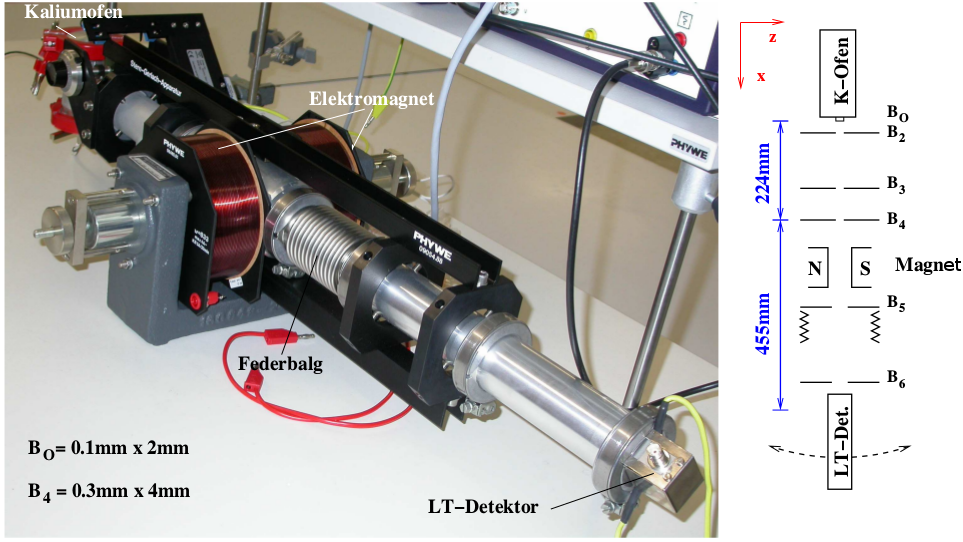
\includegraphics[height=8.5cm]{ressources/aufbau.png}
  \caption{Aufbau des Stern-Gerlach-Versuchs (links Foto, rechts Skizze) \cite{skript}.}
  \label{fig:aufbau1}
\end{figure}

Es wird ein Kalium$^{39}$-Strahl verwendet, welcher ein Blendensystem durchläuft bevor er durch ein inhomogenes Magnetfeld abgelenkt und anschließend von einem Langmuir-Taylor-Detektor detektiert wird.
Der Innenbereich des Versuchs befindet sich in einem Vakuum, gewährleistet durch eine Drehschieber- und Turbomolekularpumpe, um Stöße der Kalium-Atome mit Restgasionen zu vermeiden.
Der Kalium-Strahl wird von einem Kaliumofen emittiert.
Dieser ist in Abbildung \ref{fig:aufbau2} skizziert.
\begin{figure}
  \centering
  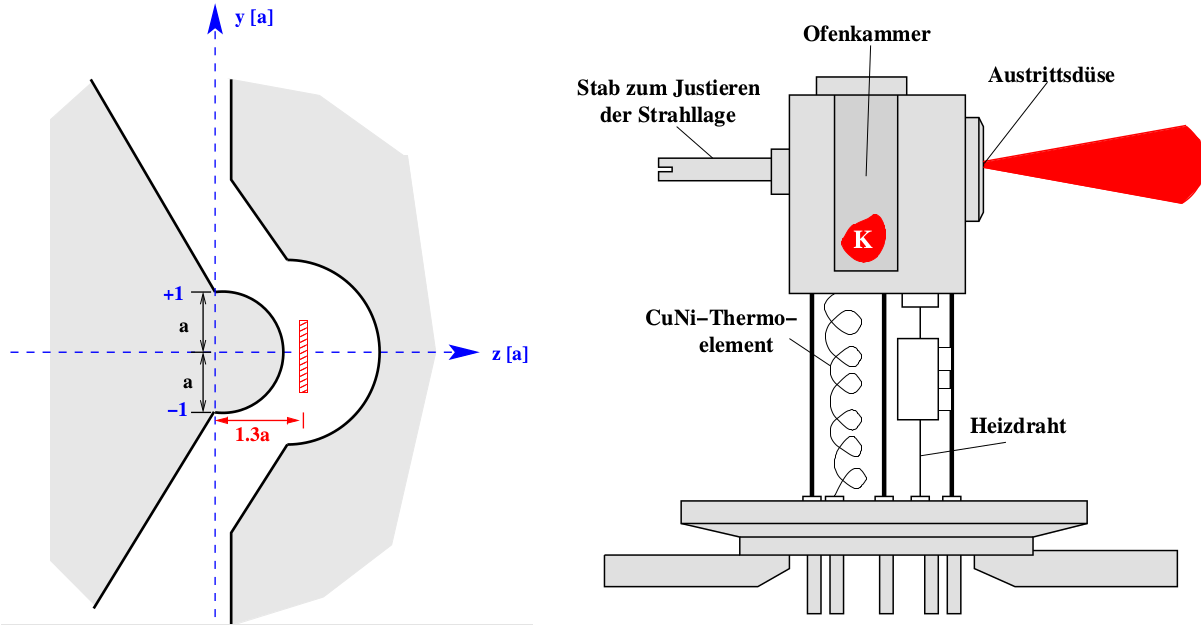
\includegraphics[height=8.5cm]{ressources/aufbau2.png}
  \caption{Links: Skizze der Polschuhe des Magneten; Rechts: Skizze des Kaliumofens \cite{skript}.}
  \label{fig:aufbau2}
\end{figure}
Das Kernstück des Versuchs bildet ein Elektromagnet mit einem zylinderförmigen Polschuhprofil, welcher in Abbildung \ref{fig:aufbau2} dargestellt ist.
Er soll einen nahezu konstanten Feldgradienten erzeugen (roter Bereich).
Daher sind die Abmessungen so gewählt, dass das Magnetfeld dessen zweier paralleler Drähte entgegengesetzter Stromrichtung mit Abstand $2a$ entspricht.
Der Bereich des konstanten Feldgradienten befindet sich in diesem Fall im Abstand von $1.3a$ zur Ausprägung der Wölbung.
Die Ablenkung der Kalium-Atome, die diesen Bereich passieren, ist proportional zum Quadrat ihrer reziproken Geschwindigkeit $s\sim \frac{1}{v^2}$.
Hierbei wird klar, dass das Vakuum einen dualen Zweck erfüllt.
Durch den geringen Druck wird die Verdampfungstemperatur von Kalium erheblich reduziert, wodurch die Austrittsgeschwindigkeit auf einen möglichst geringen Wert fällt, was, siehe \eqref{eqn:geschwindigkeit}, in einer maximalen Ablenkung im Magnetfeld resultiert.\\
Nach Passieren des Magnetfeldes gelangen die Kalium-Atome zu dem LT-Detektor, welcher sich auf einem schwenkbaren Arm befindet.
Durch die Schwenkung kann das gesamte Intensitätsspektrum in Ablenkungsrichtung aufgenommen werden.
Der LT-Detektor besteht aus von Nickel umgebenen Wolframdraht.
Die Kalium-Atome werden durch Beheizen des Wolframdrahtes als Ionen von dessen Oberfläche erneut emittiert.
